\documentclass{article}
\usepackage{graphicx}
\graphicspath{ {/home/sina/Pictures/forex} }
\usepackage[localise=on]{xepersian}
\settextfont{XB Yas}
\begin{document}
	\عنوان{فارکس}
	\عنوان‌ساز
	\صفحه‌جدید
	\فهرست‌مطالب
	\صفحه‌جدید
	\قسمت{قسمت دوازدهم بخش اول}
	\زیرقسمت{رفتار قیمت به صورت امواج}
		\پاراگراف{رفتار قیمت}
			رفتار قیمت متاثر از هیجانات، ترس ها، نگرانی ها و امید های معامله گران هست که به صورت هم‌جهت تاثیر خودش را بر روی عرضه و تقاضا میگذاره و باعث ایجاد تغیرات در قیمت میشه.
			
			\پاراگراف{قیمت چگونه تغییر میکند؟}
			اکثر معامله گران بر اساس احساساتی که بهشون دست میده و تصمیماتی که میگیرن معاملات خودشان را باز میکنند یا می‌بندند و هم جهت بودن این معاملات باعث ایجاد قیمت جدید و حرکت قیمت به یک جهت میشه
			
			\پاراگراف{تمایل یا گرایش بازار چیست و چه تاثیری در سود ما دارد؟} برای بدست آوردن سود باید تمایل بازار و معامله گران را به درستی شناخت و در آن جهت به معامله پرداخت، به تمایل و گرایش بازاد که جهت اصلی بازار به آن سمت هست را \متن‌لاتین{Market Sentiment} گفته می‌شود.  
			\پاراگراف {برای شناخت از تمایل یا گرایش بازار دو عامل مورد نیاز است:}
			\شروع{شمارش}
			\فقره{تشخیص جهت معاملات از طریق آشنایی با نمودار ها}: یعنی باید بتوان با نگاه کردن به نمودار تشخیص داد معاملات در چه جهت داره انجام میشه یا حرکت قیمت به کدام سمت است.
			\فقره{جبر بازار در مورد کالا در زمان انجام معامله از طریق اخبار و رسانه مطلع باشیم}
			\پایان{شمارش}
			برای مثال قیمت طلا در حال رشد هست و قیمت هرروز بالا میره و ما طلا داریم اگه بخواهیم همجهت با بازار رفتار بکنیم چه از نظر تکنیکال و چه از نظر اخبار و فاندامنتال ما طلا را نگهمیداریم تا زمانی که بازار از یکی از این دو عامل یا دو جنبه دچار نقصان یا ضعف شده
		\زیرزیرقسمت{حرکت قیمت به صورت موج }
		نحوه رفتار قیمت بر روی نمودار به صورت ترکیبی از \متن‌سیاه{امواج} و شناخت جهت تمایل امواج از مهمترین عوامل موفقیت در بازار های مالی است در واقع جهت معامله معامله گران بزرگ\\
		\زیرزیرقسمت{حرکت جنبشی و اصلاحی}
		حرکت قیمت: جنبشی، اصلاحی\\
		\پاراگراف{حرکت جنبشی یا Movement} حرکتی که در آن قیمت در جهت اصلی روند انجام می‌دهد که معمولا با شتاب و انرژی زیادی همراه است
		
		
		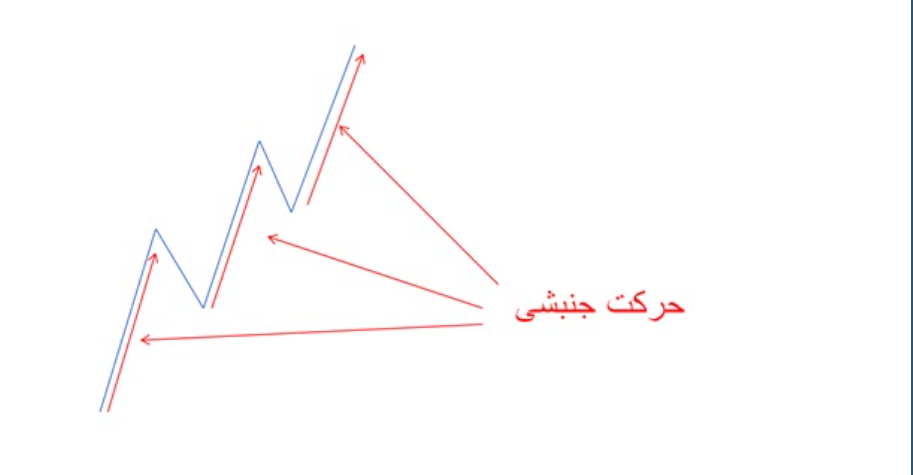
\includegraphics[width=8cm, height=4cm]{pics/حرکت جنبشی.png}
				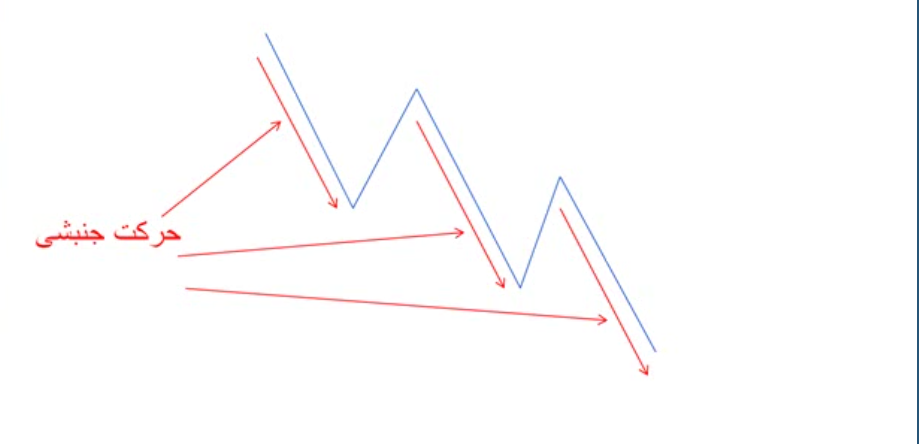
\includegraphics[width=8cm, height=4cm]{pics/حرکت جنبشی نزولی.png}
		
		\پاراگراف{حرکت اصلاحی یا Retracement}
		قیمت پس از حرکت جنبشی و خسته شدن انجام میدهد و خلاف جهت حرکت جنبشی و روند اصلی هست که نشان میدهد قیمت نیاز دارد که استراحت کند و انرژی جمع کنه برای حرکت در جهت روند اصلی

		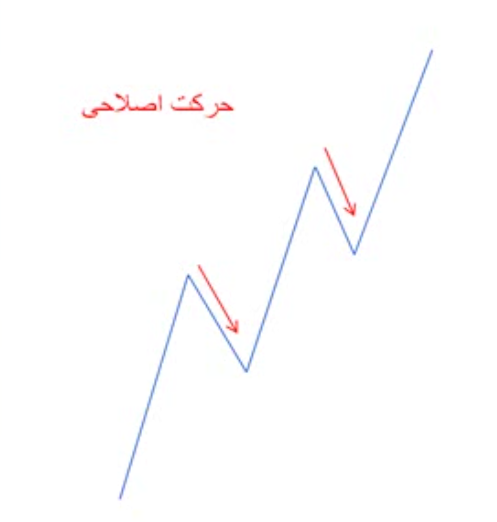
\includegraphics[width=5cm, height=4cm]{pics/حرکت اصلاحی.png}


		بعد از های جدید(سطح های جدید) بعد هجوم و خرید رشد بعد 
		از نقد کردن سود افت\\
	\زیرزیرقسمت{روند خنثی \متن‌لاتین{Neutral Trend}} جهت خاثی ندار و معامله‌گران هیج کاری 			نمیکنند فقط  حرکت اصلاحی است و بدون حرکت جنبشی است\\
		
		\زیرزیرقسمت{نقاط بالایی(Highs) و پایینی(Lows)}
		
		\زیرزیرقسمت{تشخیص روند صعودی و نزولی}
		نقطه higher high یا HH زمانی که hh و hl داریم روند صعودی هست\\
		در روند صعودی هایر های پشت سر هم داریم \\
		
		\زیرزیرقسمت{تشخیص یک روند و یک اصلاحی}
		با استفاده از هایر ها و لور ها جنبشی یا اصلاحی بودن حرکت
		را تشخیص داد 
	
	
	\قسمت{قسمت دوازده بخش ۲}
	\زیرقسمت{تشخیص اتمام روند}
		تشخیص به موقع به این دلیل مهم هست که شخص میتواند پوزیشن های بازش رو
		تسویه کنه و سودش رو از بازار بکشه بیرون یا از پوزشن های
		خلاف جهت که احتمال داره بهش ضرر برسونه جلوگیری کنه
		\زیرزیرقسمت{دو عامل اصلی اخطار های تغییر روند}
		\شروع{شمارش}
			\فقره عدم توانایی قیمت در تشکیل های جدید در روند صعودی یا لو در روند نزولی
			\فقره شکسته شدن اخرین لو در روند های صعودی یا اخرین 
			های در روند های نزولی 
		\پایان{شمارش}
		
		\قسمت{قسمت دوازده بخش ۳}
			\زیرقسمت{الگو دو سقف \متن‌لاتین{Double Top}}
			\زیرقسمت{اندازه اصلاحی ها نسبت به حرکت جنبشی}
				مقدار های ۱/۳ ، ۱/۲ یا ۲/۳
		
	
	
\end{document}